\documentclass[12pt]{article}

\usepackage{sbc-template}

\usepackage{graphicx,url}

\usepackage[brazil]{babel}   
%\usepackage[latin1]{inputenc}  
\usepackage[utf8]{inputenc}  
\usepackage{listings}
\usepackage{float}
\usepackage{amsmath}
\usepackage{amssymb}
% UTF-8 encoding is recommended by ShareLaTex

\usepackage{color}
\definecolor{javared}{rgb}{0.6,0,0} % for strings
\definecolor{javagreen}{rgb}{0.25,0.5,0.35} % comments
\definecolor{javapurple}{rgb}{0.5,0,0.35} % keywords
\definecolor{javadocblue}{rgb}{0.25,0.35,0.75} % javadoc

\lstset{language=Java,
	basicstyle=\ttfamily,
	keywordstyle=\color{javapurple}\bfseries,
	stringstyle=\color{javared},
	commentstyle=\color{javagreen},
	morecomment=[s][\color{javadocblue}]{/**}{*/},
	numbers=left,
	numberstyle=\tiny\color{black},
	stepnumber=1,
	numbersep=5pt,
	tabsize=2,
	showspaces=false,
	showstringspaces=false}
     
\sloppy

\title{Controle de segurança para cartões de crédito usando K-Means}

\author{Fabrícia de Jesus Santos\inst{1}, \\ Thiago Alessandro dos Santos Pereira\inst{1}, Weslley Henrique Campos Santos\inst{1}}


\address{Departamento de Sistemas de Informação \\Universidade Federal de Sergipe (UFS) -- Itabaiana, SE -- Brasil\\
  \email{fabriciacooper@gmail.com}
  \email{thi.alessandro@hotmail.com, weslley$\_$campos@outlook.com}
}

\begin{document} 

\maketitle

\section{Introdução}
Devido a grande ocorrência de clone de cartões de crédito e débito, as empresas de cartão investem como mitigar esse tipo de crime. Recentemente, nos Estados Unidos passaram do uso da faixa magnética insegura em cartões de crédito e débito para cartões de chip e PIN mais bem protegidos, regulados pelo padrão EMV.

Aqui no Brasil o uso de cartões com chips já vem acontecendo alguns anos, porém pesquisadores descobriram que cibercriminosos brasileiros desenvolveram uma maneira de roubar dados e clonar cartões de chip e PIN. Na maioria dos casos, as vítimas não são informadas no seu devido tempo, ocasionando um transtorno, sendo que em alguns casos são solucionáveis e em outros não.

Geralmente, as empresas tentar informar aos seus clientes como manter-se informado sobre alguma anormalidade. Entre essas informações estão:
\begin{enumerate}
	\item Verificar histórico de transações do cartão;
	\item Utilizar aplicativo como AndroidPay ou o ApplePay para não revelar os dados do seu cartão;
	\item Ter bastante cuidado ao realizar compras pela internet, pois é possível encontrar sites fraudados que podem roubar os dados;
\end{enumerate}

O Brasil é um dos países campeões de fraude on-line, dentre outros motivos, por ter sido também um dos pioneiros na adoção do cartão chipado, que promove um alto grau de segurança para transações presenciais. Com o desuso da tarja magnética nos sistemas de pagamentos, os golpes migraram para a internet, tornando e-commerce um dos mais vulneráveis do planeta.
\section{Objetivo}
O objetivo do projeto é apresentar uma aplicação mobile que monitore as compras do consumidor ao usar seu cartão de crédito. Utilizando a aplicação, a pessoa poderá receber uma notificação, caso existe alguma compra realizada fora do padrão. Dessa forma, a própria pessoa estará informada sobre suas transições, e caso seja identificado alguma anormalidade, a vitima poderá entrar em contato com a empresa de cartão de crédito para tomar as medidas cabíveis.

A aplicação adota algoritmo K-means, que será explicado logo em seguida.
\section{K-means}
K-means é um tipo de aprendizado não supervisionado, que é usado quando você tem dados sem rótulo, ou seja, dados sem categorias ou grupos definidos. O objetivo deste algoritmo é encontrar grupos, sendo que o número de grupos é representado pela variável K. O algoritmo funciona iterativamente para atribuir cada ponto de dados a um dos grupos K com base nos recursos fornecidos. Os pontos de dados são agrupados com base na similaridade do recurso. Os resultados do algoritmo de agrupamento K-means são:

\begin{itemize}
	\item Os centroídes dos clusters K, podem ser usados para rotular novos dados; 
	\item Etiquetas para os dados de treinamento (cada ponto de dados é atribuído a um único cluster).
\end{itemize}

Em vez de definir grupos antes de examinar os dados, o armazenamento em cluster permite localizar e analisar os grupos que foram formados organicamente. Cada centroide de um cluster é uma coleção de valores de recursos que definem os grupos resultantes. Examinar os pesos dos recursos do centróide pode ser usado para interpretar qualitativamente o tipo de grupo que cada cluster representa. 

\subsection{Uso no ramo de negócios}
O algoritmo K-means é usado para localizar grupos que não foram explicitamente rotulados nos dados. Isso pode ser usado para confirmar suposições de negócios sobre quais tipos de grupos existem ou para identificar grupos desconhecidos em conjuntos de dados complexos. Depois que o algoritmo é executado e os grupos são definidos, qualquer novo dado pode ser facilmente atribuído ao grupo correto.

Este é um algoritmo versátil que pode ser usado para qualquer tipo de agrupamento. Alguns exemplos de casos de uso são:

\begin{itemize}
	\item Segmentação comportamental:
	\begin{itemize}
		\item Segmentar por histórico de compras;
		\item Segmento por atividades no aplicativo, site ou plataforma;
		\item Definir personas com base em interesses;
		\item Criar perfis com base no monitoramento de atividades.
	\end{itemize}
\end{itemize}

\begin{itemize}
	\item Categorização de inventário:
	\begin{itemize}
		\item Inventário do grupo por atividade de vendas;
		\item Inventário do grupo por métricas de produção;
	\end{itemize}
\end{itemize}

\begin{itemize}
	\item Classificando as medições do sensor:
	\begin{itemize}
		\item Detectar tipos de atividade em sensores de movimento;
		\item Agrupar imagens;
		\item Áudio separado;
		\item Identificar grupos no monitoramento de integridade;
	\end{itemize}
\end{itemize}

\begin{itemize}
	\item Detectando bots ou anomalias:
	\begin{itemize}
		\item Separe os grupos de atividades válidos dos bots;
		\item Agrupar atividade válida para limpar a detecção de outliers.
	\end{itemize}
\end{itemize}

Além disso, o monitoramento se um ponto de dados rastreado alterna entre grupos ao longo do tempo pode ser usado para detectar alterações significativas nos dados.
\subsection{Algoritmo}
O K-means usa refinamento iterativo para produzir um resultado final. As entradas do algoritmo são o número de clusters K e o conjunto de dados. O conjunto de dados é uma coleção de recursos para cada ponto de dados. Os algoritmos começa com estimativas iniciais para os k  centroides, que podem ser geradas aleatoriamente ou aleatoriamente selecionados a partir do conjunto de dados. O algoritmo então itera entre duas etapas.
\subsubsection{1ª Etapa de avaliação dos dados}
Cada centróide define um dos clusters. Nesta etapa, cada ponto de dados é atribuído ao seu centróide mais próximo, com base na distância euclidiana ao quadrado. Mais formalmente, se c$_{i}$ é a coleção de centróides no conjunto \textit{C}, então cada ponto de dados \textit{x} é atribuído a um cluster com base.
\begin{figure}[H]
	\centering
	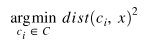
\includegraphics[width=0.20\columnwidth]{imagem/formula}
\end{figure}
Onde \textit{dist}( ) é a distância euclidiana padrão (L$_{2}$). Deixa o conjunto de atribuições de pontos de dados para cada i$^{th}$ centróide aglomerado ser S$_{i}$.
\subsubsection{2ª Etapa de atualização do centroíde}
Nesta etapa, os centroides são recalculados. Isso é feito tomando a média de todos os pontos de dados atribuídos ao cluster desse centróide.
\begin{figure}[H]
	\centering
	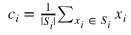
\includegraphics[width=0.20\columnwidth]{imagem/formula2}
\end{figure}
O algoritmo itera entre as etapas um e dois até que um critério de parada seja atendido, ou seja, nenhum ponto de dados altera os clusters, a soma das distâncias é minimizada ou algum número máximo de iterações é atingido.

Este algoritmo é garantido para convergir para um resultado. O resultado pode ser um ótimo local, não necessariamente o melhor resultado possível, o que significa que a avaliação de mais de uma execução do algoritmo com centróides de partida randomizados pode dar um resultado melhor.
\subsection{Escolhendo o K}
O algoritmo descrito acima encontra os clusters e rótulos de conjunto de dados para um K pré-escolhido em particular. Para encontrar o número de clusters nos dados, precisa executar o algoritmo para um intervalo de  valores K e comparar os resultados. Em geral, não há um método para determinar o valor exato de K, mas uma estimativa precisa pode ser obtida usando as seguintes técnicas.

Uma das métricas comumente usadas para comparar os resultados em diferentes valores de K é a distância média entre os pontos de dados e seu centróide de cluster. Desde o aumento do número de clusters sempre reduzir a distância de pontos de dados, aumentando a K irá sempre diminuir essa métrica, ao extremo de se chegar a zero quando K é o mesmo que o número de pontos de dados. Assim, essa métrica não pode ser usada como o único destino. Em vez disso, a média de distância para o baricentro como uma função de K é plotado e o ``ponto de cotovelo'', onde a taxa de diminuição muda bruscamente, pode ser usado para determinar aproximadamente K.

Existem várias outras técnicas para validação de K, incluindo validação cruzada, critérios de informação, o método de salto teórico de informação, o método de silhueta e o algoritmo de G-médias. Além disso, o controlo da distribuição de pontos de dados entre os grupos fornece informações sobre a forma como o algoritmo é dividir os dados para cada K.

\section{Aplicação}

\section{Conclusão}
O presente projeto teve por objetivo aplicar o algoritmo de K-means sobre o problema citado anteriormente. O maior propósito é ganhar conhecimento sobre a área de Inteligência Artificial e ter suporte para aplicar os seus conceitos. Contudo, deve ser realizado um estudo mais aprofundado para solucionar de forma eficaz o problema. 

O número de ocorrências sobre cartões clonados vem aumentando cada vez mais, dessa forma, muitas empresas investem para mitigar esse tipo de ameaça que traz grandes prejuízos ao consumidor. Adotando a ideia sugerida no projeto, a vítima ficará informada sobre alguma anormalidade.

Apesar da complexidade de utilizar K-means, este é o melhor algoritmo para solucionar o problema abordado.
\end{document}
